%\section{Title @Venue'Year}
%\subsection{Background/Problems}
%\subsection{Methods/Techniques}
%\subsection{Results/Evaluation}
%\subsection{Limitations/My Comments}
%\newpage
\documentclass[]{article} %twocolumn
%\usepackage{ctex}
\usepackage{titlesec}
\titleformat*{\section}{\large\bfseries} %\tiny\scriptsize\footnotesize\small\normalsize\large\Large\LARGE\huge\Huge
\titleformat*{\subsection}{\normalfont\bfseries}
\usepackage{graphicx}
\usepackage{url}
\usepackage{listings}
\usepackage[a4paper,margin=2cm]{geometry}
%\geometry{a4paper,left=2cm,right=2cm,top=1cm,bottom=1cm}
%\special{papersize=5in,8in} %dvi 没有纸张大小的概念,只有转换成 .ps、.pdf 文件时,才由对应的输出驱动(如 Dvips、dvipdfmx 或 pdfTeX 等)设置输出纸张大小。
%传统的 TeX 代码里面本身不能直接设置纸大小,因此才需要在安装 TeX Live 时选择那些输出驱动的默认纸张大小。而 article 等文档类的 a4paper、letterpaper 选项,只是设置合适的版心位置和距离,以适合这些纸张大小。
%不过,在 TeX 代码里面用特定输出驱动的 special 命令,可以提示这些输出驱动选择纸张,一般用 geometry 宏包的话,就会处理这个问题。而 graphics 宏包后台对 pdfTeX 也有相应的代码(在 pdftex.def 中)。
%\setcounter{secnumdepth}{3}		%编号深度
\setcounter{tocdepth}{1}		%目录深度


\title{\textbf{Reading Notes of Recent Papers}}%文献阅读笔记
\author{\texttt{TSIS Lab.} (Trusted Software and Intelligent System Lab.)}
\date{2020/01/21} %如果没有这行将显示当前时间, 如果不想显示时间则使用 \date{}

\begin{document}

\maketitle     %生成标题, 包括 \title \author \date
\tableofcontents  %生成目录
\clearpage

\twocolumn
\section{SAVIOR: Towards Bug-Driven Hybrid Testing @S\&P'20
}
\subsection{Background/Problems}
%\subsection{Methods/Techniques}
%\subsection{Results/Evaluation}
%\subsection{My Comments}
Hybrid testing combines fuzzing and concolic
execution. It leverages fuzzing to test easy-to-reach code
regions and uses concolic execution to explore code blocks
guarded by complex branch conditions. As a result, hybrid testing
is able to reach deeper into program state space than fuzz
testing or concolic execution alone. Recently, hybrid testing has
seen significant advancement. However, \textbf{its code coverage-centric
design is inefficient in vulnerability detection}. First, it \textbf{blindly}
selects seeds for concolic execution and aims to explore new code
continuously. However, as statistics show, a large portion of the
explored code is often bug-free. Therefore, giving equal attention
to every part of the code during hybrid testing is a non-optimal
strategy. It slows down the detection of real vulnerabilities by
over 43\%. Second, classic hybrid testing quickly moves on after
reaching a chunk of code, rather than examining the hidden
defects inside. It may frequently \textbf{miss subtle vulnerabilities}
despite that it has already explored the vulnerable code paths.
\subsection{Methods/Techniques}
We propose SAVIOR (Fig.\ref{fig:savior}), a new hybrid testing framework pioneering
a bug-driven principle.

\textbf{Bug-driven prioritization:} Instead of running all seeds without
distinction in concolic execution, SAVIOR prioritizes
those that have higher possibilities of leading to vulnerabilities.
Specifically, before the testing, SAVIOR analyzes the source
code and \textbf{statically labels the potentially vulnerable locations}
in the target program.
Moreover, SAVIOR computes the set of basic blocks reachable
from each branch. During dynamic testing, SAVIOR \textbf{prioritizes the concolic execution seeds that can visit more
important branches} (i.e., branches whose reachable code has
more vulnerability labels).

\textbf{Bug-guided verification: }Aside from accelerating vulnerability
detection, SAVIOR also verifies the labeled vulnerabilities
along the program path traversed by the concolic executor.
Specifically, SAVIOR synthesizes the faulty constraint of
triggering each vulnerability on the execution path. If such
constraint under the current path condition is satisfiable,
SAVIOR solves the constraint to construct a test input as
the proof. Otherwise, SAVIOR proves that the vulnerability
is infeasible on this path, regardless of the input.

\begin{figure*}[t]
    \centering
    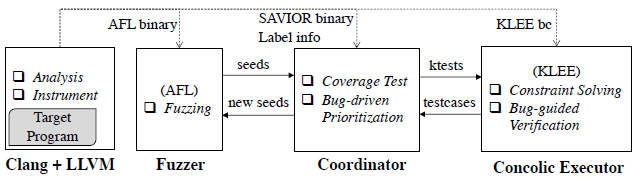
\includegraphics[scale=0.9]{savior.png} %
    \caption{SAVIOR's arch.}	
    \label{fig:savior}
\end{figure*}

\subsection{Results/Evaluation %评估效果
}
Our evaluation shows that the bug-driven approach outperforms mainstream
 hybrid testing systems driven by code coverage. On average, SAVIOR
detects vulnerabilities 43.4\% faster than DRILLER and 44.3\%
faster than QSYM, leading to the discovery of 88 and 76 more
unique bugs, respectively. According to the \textbf{evaluation on 11 well
fuzzed benchmark programs, within the first 24 hours, SAVIOR
triggers 481 UBSAN violations, among which 243 are real bugs.}

\subsection{Limitations/My Comments}
\begin{itemize}
    \item Over-approximation in Vulnerability Labeling: SAVIOR leverages sound algorithms
to label vulnerabilities where the over-approximation may
introduce many false-positive labels. This imprecision can
consequently weaken the performance of SAVIOR's prioritization. 
We plan to include more precise
static analysis for finer-grained label pruning.
    \item Prediction in Vulnerability Detection: Once reaching a
potentially vulnerable location in concolic execution,
SAVIOR extracts the guarding predicates of the vulnerability
label. However, these predicates may contradict the current
path condition. In case of such contradiction, SAVIOR terminates
the exploration of the labeling site immediately.
Moreover, we can predict whether an execution
path can trigger a vulnerability or not by studying the
runtime information of previous executions, more importantly,
before that execution arrives the vulnerability site. To
achieve this goal, we need to backwardly summarize
path constraints from the labeled site to its predecessors in
the explored paths, by using the weakest precondition.
    \item Hybrid testing in SAVIOR is same with hybrid fuzzing in Driller and Berry. Both tools run fuzzing for code exploration and invoke concolic execution only on
hard-to-solve branches, which takes advantage of both fuzzer's
efficiency and concolic executor's constraint solving.
\end{itemize}
\newpage
\section{Fuzzing File Systems via Two-Dimensional Input Space Exploration @S\&P'19}
\subsection{Background/Problems}
File systems are too big and too complex to be bug free. Nevertheless, to find bugs in file systems, regular stress-testing tools and formal checkers are limited due to the ever-increasing complexity of both file systems and OSes. Thus, fuzzing becomes a preferable choice, as it does not need much knowledge about a target. However,
three prominent issues of existing file systems fuzzers exist: 
(1) fuzzing a large blob image is inefficient; 
(2) fuzzers do not exploit the dependence
between a file system image and file operations; 
(3) fuzzers use aging OSes and file systems, which results in
irreproducible bugs.

\subsection{Methods/Techniques}
we present JANUS (Fig.\ref{fig:janus}, 120K C++/C LoC), the first feedback-driven fuzzer
that explores the two-dimensional input space of a file system,
i.e., mutating metadata on a large image, while emitting image-directed
file operations. In addition, JANUS relies on a library
OS rather than on traditional VMs for fuzzing, which enables
JANUS to load a fresh copy of the OS, thereby leading to better
reproducibility of bugs.
\begin{figure}[h]
    \centering
    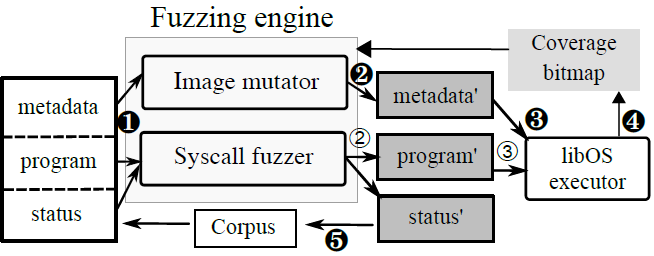
\includegraphics[scale=0.5]{janus.png} %
    \caption{JANUS' arch.}	
    \label{fig:janus}
\end{figure}
\subsection{Results/Evaluation}
We evaluate JANUS on 8 file systems
and found 90 bugs in the upstream Linux kernel, 62 of which have
been acknowledged. 43 bugs have been fixed with 32
CVEs assigned. In addition, JANUS achieves higher code coverage
on all the file systems after fuzzing 12 hours, when compared
with the state-of-the-art fuzzer Syzkaller.
JANUS visits 4.19X and 2.01X more code paths in Btrfs and ext4,
respectively. Moreover, JANUS is able to reproduce 88–100\% of
the crashes, while Syzkaller fails on all of them.
\subsection{Limitations/My Comments}
\begin{itemize}
    \item JANUS cannot fuzz the DAX mode of a file system without modification on LKL. 
    \item To achieve a minimal PoC, JANUS uses a brute force approach to revert
every mutated byte and also tries to remove every invoked
file operation to check whether the kernel still crashes at the
expected location, which is sub-optimal.
    \item JANUS does not support file systems (e.g., NTFS, GVfs, SSHF, etc.)
that rely on FUSE (Filesystem in Userspace).
    \item By combining Janus and kAFL, we can fuzz file systems on other OSes.
    \item Other crash-consistency checkers [6,73] and semantic correctness checkers [36, 58] can rely on or integrate with Janus which aims to find general security bugs in file systems.
    \item To find security bugs in OSes, a number
    of general kernel fuzzing frameworks [20, 43, 46, 61] and
    OS-specific kernel fuzzers [22, 25, 44, 45, 47] have been
    proposed. Unlike JANUS, all these fuzzers generate random
    system calls based upon predefined grammar rules, which is
    ineffective in the context of file system fuzzing. Several recent
    OS fuzzers such as IMF [22] and MoonShine [49] focusing
    on seed distillation are orthogonal to this work. Nevertheless,
    JANUS can start with seed programs of high quality by utilizing
    their approaches.
\end{itemize}
\newpage
\section{REDQUEEN: Fuzzing with Input-to-State Correspondence @NDSS'19}
\subsection{Background/Problems}
Two common problems of fuzzing are magic numbers
and (nested) checksums (see Listing \ref{fuzzissues}). Computationally expensive methods such
as taint tracking and symbolic execution are typically used to
overcome such roadblocks. Unfortunately, such methods often
require access to source code, a rather precise description of the
environment (e.g., behavior of library calls or the underlying OS),
or the exact semantics of the platform's instruction set, and thus 
such methods are the polar opposite of the approach pioneered by AFL: to a
large extend, AFL's success is based on the fact that it makes
few assumptions about the program's behavior.
\begin{lstlisting}[label=fuzzissues,language={[ANSI]C}, caption={Roadblocks for feedback-driven fuzzing.}]
/* magic number example */
if(u64(input)==u64("MAGICHDR"))
  bug(1);
/* nested checksum example */
if(u64(input)==sum(input+8, len-8))
  if(u64(input+8)==sum(input+16, len-16))
    if(input[16]=='R' && input[17]=='Q')
      bug(2);
\end{lstlisting}

\subsection{Methods/Techniques}
We introduce a lightweight, yet very effective
approach to facilitate
and optimize state-of-the-art feedback fuzzing that easily scales
to large binary applications and unknown environments. We
observe that during the execution of a given program, parts
of the input often end up directly (i.e., nearly unmodified)
in the program state. This \emph{input-to-state correspondence} can
be exploited to create a robust method to overcome common
fuzzing roadblocks in a highly effective and efficient manner.
Our prototype implementation, called REDQUEEN, is able to
solve magic bytes and (nested) checksum tests automatically
for a given binary executable. Additionally, we show that our
techniques outperform various state-of-the-art tools on a wide
variety of targets across different privilege levels (kernel-space
and userland) with no platform-specific code.
\subsection{Results/Evaluation}
REDQUEEN (\url{https://github.com/RUB-SysSec/redqueen}) is the
first method to find more than 100\% of the bugs planted in
LAVA-M across all targets. Furthermore, we were able to discover
65 new bugs and obtained 16 CVEs in multiple programs and
OS kernel drivers. Finally, our evaluation demonstrates that
REDQUEEN is fast, widely applicable and outperforms concurrent
approaches by up to three orders of magnitude.

\subsection{Limitations/My Comments}
\begin{itemize}
    \item REDQUEEN cannot deal with those cases in which the input does not correspond to the state, such as compression or hash maps in the input.
    \item It would be beneficial to use this
lightweight approach as a first step where possible, and than
solve the remaining challenges using complex approaches.
\end{itemize}
\end{document}
